% !TEX root = ../Masters.tex
\chapter{Evaluation of DGEL}
DGEL consists of to main modules: \textit{generation} and \textit{evaluation}.
The evaluation module consists of the fitness component which evaluates who good the L-system plants are.
The remaining components are part of the generation component which generates plants, and uses the evaluation module to generate \textit{good} plants.
To answer if DGEL solves the research questions, both modules have to be evaluated.
The generation module will be evaluated in a technical manner to determine if it performs well or not.
The evaluation module will be evaluated using humans as to answer if the fitness function properly rates plants as aesthetically pleasing or not.

\section{Evaluation of the Generation Module}
\subsection{Method}
As explained in Section~\ref{sec:overview} and shown in Figure~\ref{fig:dgel}, there are two main processes involved in generating the model for the L-system plants: \textit{SA} and \textit{GE}.
The remaining steps are dependent on the model and do not create variations on the same model.
Thus GE and SA are the two processes of interests to evaluate.

% SA progress - have data, though not structured
% SA random vs random - have data, need plot.
% GE SA vs GE uniform - need data, how to measure?
% Comparing plants from different SA.

\subsubsection{Grammar Evolution}
GE, as with GA, depends on multiple parameter, and with tournament sampling there are even more.
Thus, before evaluation the GE process, good parameters had to be found.
Additionally, seeing what parameters are needed for a good performing GE may reveal additional properties of it.
The parameters were found using a combined manual and automated approach by searching the parameter space in multiple steps.
The idea was not to find the optimal parameters, but rather to find some parameters that made the GE produce an individual with good fitness within a reasonable time.
It was assumed that the size parameters -- population size and number of generations -- are the baseline parameters for GE and thus should be found first.
Then the tournament size for the tournament selection strategy should be found.
Then good parameters for the recombination rates -- crossover rate and mutation rate -- should be found.
Finally the parameter for the GE gene duplication operator should be found.

To search for the GE parameters, a breadth-first graph search inspired approach was used.
An example is shown in Figure~\ref{fig:parameter-search}.
The approach tests a combination of parameters by doing 20 GE runs with those parameters and using the mean fitness score of the best individual from each run.
If the score is an improvement of the previous score, the search will also tests the neighboring nodes in the graph by increasing the parameter values.
Otherwise, the current parameter values will be considered as not improving the performance and thus be discarded.
When there are no more improvements, the parameter values that produced the best score will be returned.
The parameter values will start at a small value and increase in an exponential fashion.
This is based on the assumption that the parameters are more sensitive when the values are small.
All of the parameter searches, except for the reproduction parameter search, will increase with a multiplicative of 2.
Because the reproduction rate parameters are bounded ($[0, 1]$) and to cover the whole range with a reasonable amount of steps, custom steps of 0.01, 0.1, 0.5 and 1 were used.

\begin{figure}
    \centering
    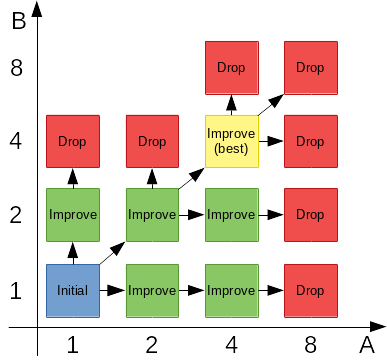
\includegraphics[width=0.6\textwidth]{figures/parameter-search}
    \caption{Example of a GE parameter search}
    \label{fig:parameter-search}
\end{figure}

To evaluate the GE process, it was compared to completely random set of L-systems.
If the best individual from the GE process has a higher fitness score than the best individual from the random set of individuals, the GE process is an improvement.
To make a fair comparison, the random set of individuals should contain as many individuals as the GE generates and modifies (through mutation or crossover)
This way, both methods will ``generate'' the same amount of individuals, either being completely new individuals or modifications of existing individuals.
GE uses a fixed number of generations and population size, resulting into a fixed number of chromosome generations and modifications: $individuals = population + population * generations$.
Thus the random set method will generate $individuals$ individuals.

Because both methods depend on a random seed, an average of multiple runs will have to be used.
A sample size of 11 was selected as balanced choice between sample size and duration.
Student's t-test was used to test the group mean difference.

\subsubsection{Simulated Annealing}
To evaluate the SA process, a list of questions were made:
\begin{itemize}
	\item Can SA and the grammar distribution be used to find portions of the parameter space that generate better L-system plants?
	\item Does SA enable GE to find better L-system plants?
	\item Can SA find multiple portions of the parameter space that each generate unique-looking plants?
\end{itemize}
To answer the first question, two methods were used.
First, SA was used as described in previous sections to find an optimized distribution, and the progress of it was plotted.
The progress plot was analyzed to see if SA made any meaningful progress.
Secondly, a comparison was made between the average fitness of L-systems randomly generated by a uniform distribution and L-systems randomly generated by an SA-optimized distribution.
The L-systems were generated in a completely random manner, not using any evolutionary approach such as GE.
% I need to actually run this experiment....
While this may answer if it is possible for an SA-optimized distribution to generate better plants, it does not answer if this always will be the case.

To answer the second question, the performance of GE with a uniform distribution was compared to the performance of GE with an SA-optimized distribution.
Both GE processes were run 11 times, each time extracting the best L-system, before taking the mean of the best L-systems and using a t-test to test if the means were different.

\subsection{Results}
Figure~\ref{fig:size-sampling} shows the search of the population size and number of generations to be used for the GE process.
The search was prematurely stopped because at around either 1600 number of generations or population size the duration became unreasonable long.
As seen, a minimum of either a population size of 200 or 200 generations is required for a reasonable performance.
Additionally, for any number of generations, a population size of 200 makes a notable improvement.
From this point, there is a steady improvement from around 0.8 to 0.9 with both parameters increasing towards 1600.
Outside a line drawn through 800, 400 and 400, 800 there does not seem to be any notable improvement, while the duration increases by a large amount.
The parameter values that yielded the best fitness was $generations = 200$ and $population size = 800$, and they did it within a reasonable duration.
The duration of it is significantly smaller than other parameter values that yield approximately the same fitness.
Thus, these parameter values were selected for use.

\begin{figure}
    \centering
    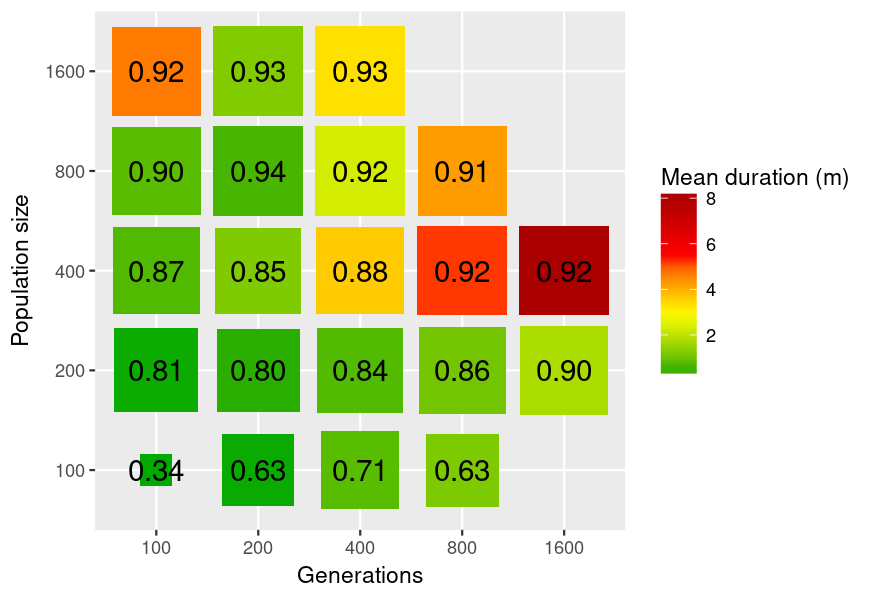
\includegraphics[width=0.8\textwidth]{figures/ge-size-sampling}
    \caption[Visualized search of GE population size and number of generations]{Visualized search of GE population size and number of generations. Numbers are the mean of best fitness scores, box sizes are a representation of that number, and colors represent the mean duration of the GE.}
    \label{fig:size-sampling}
\end{figure}

Figure~\ref{fig:tournament-sampling} shows the search of the tournament size.
Contrasted to the other searches, this is a one-dimensional search.
% Possibly do a significance test. Need to re-run to generate raw data...
As seen in the figure, the search did not find any improvements at all.
% A BIG LIMITATION IS THAT A LARGER TOURNAMENT SIZE MAY ENABLE SMALLER SIZE PARAMETERS.
Thus the tournament size was kept at the lowest value, i.e.\ 2.

\begin{figure}
    \centering
    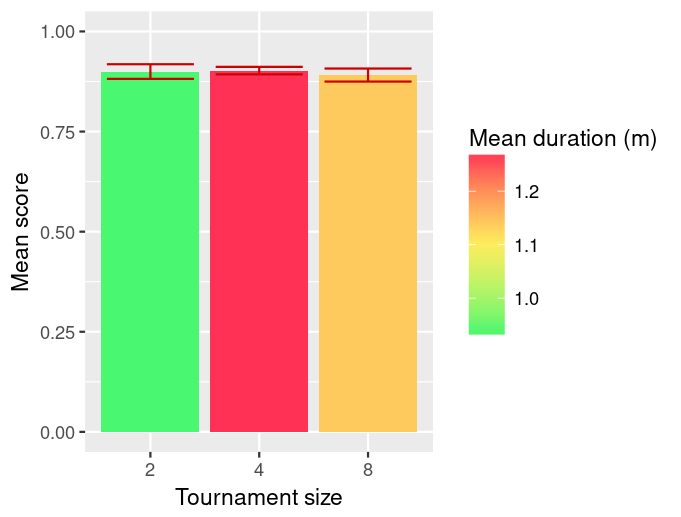
\includegraphics[width=0.7\textwidth]{figures/ge-tournament-sampling}
    \caption{Visualized search of the GE tournament selection tournament size}
    \label{fig:tournament-sampling}
\end{figure}

Figure~\ref{fig:recombination-sampling} shows the search of the recombination parameters: mutation rate and crossover rate.
There is a general improvement in fitness with both increasing mutation rate and crossover rate until the crossover rate reaches 1 where it suddenly turns for the worse.
Thus the crossover rate should at least be below 1.
Additionally, the crossover rate seems to be the parameter that contributes less to an improved fitness and increases the duration the most.
Thus the mutation rate should be the most important parameter.
The best fitness score is provided by a mutation rate of 1 and crossover rate of 0.5, further indicating this.

Figure~\ref{fig:recombination-sampling-variance} Shows the same standard deviations in the same search.
The pattern is similar to that of the mean fitness scores.
The most stable performance is provided by a mutation rate of 1 and crossover rate of 0.5.
Thus the recombination parameters will be using these values.

\begin{figure}
    \centering
    \begin{subfigure}{0.57\textwidth}
        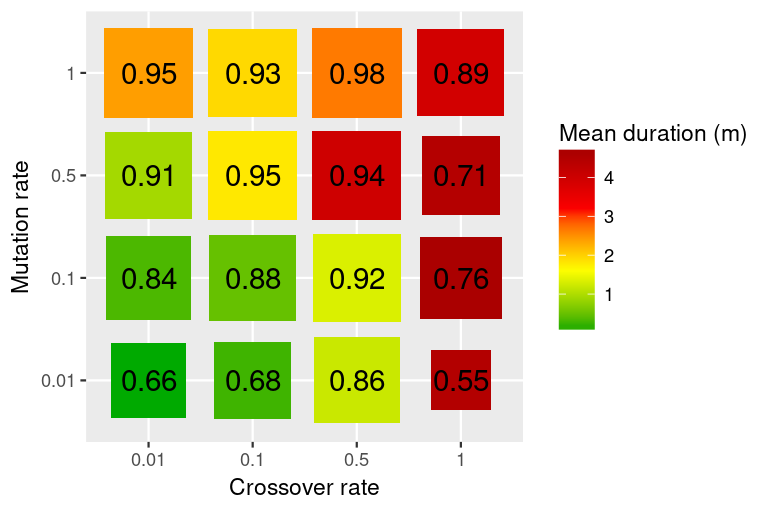
\includegraphics[width=\textwidth]{figures/ge-recombination-sampling}
        \caption{Mean of best fitness scores as numbers and sizes, with duration as colors}
        \label{fig:recombination-sampling}
    \end{subfigure}
    ~
    \begin{subfigure}{0.4\textwidth}
        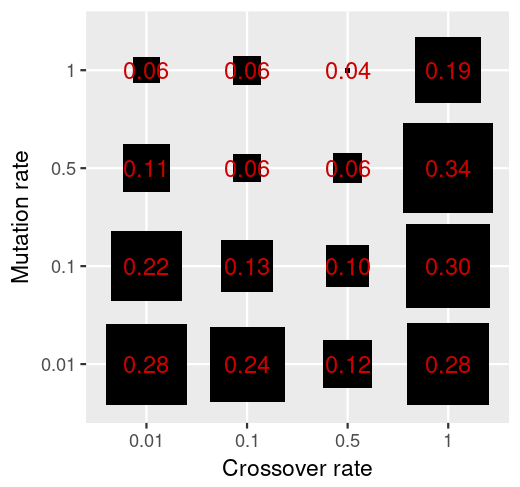
\includegraphics[width=\textwidth]{figures/ge-recombination-sampling-variance}
        \caption{Standard deviation}
        \label{fig:recombination-sampling-variance}
    \end{subfigure}
    \caption{Visualized search of the GE recombination parameters}
\end{figure}

Figure~\ref{fig:ge-random} shows the comparison of GE against random samples.
The difference in mean of best fitness is 0.13 (p < 0.01), where GE has a higher mean than random.
Thus there is a statistically significant difference between their performances.
Additionally, Figure~\ref{fig:ge-random-duration} shows the mean duration of the methods where GE is 5 times faster than random.
This indicates that GE is indeed an improvement of randomly generating samples.

\begin{figure}
    \centering
    \begin{subfigure}{0.4\textwidth}
        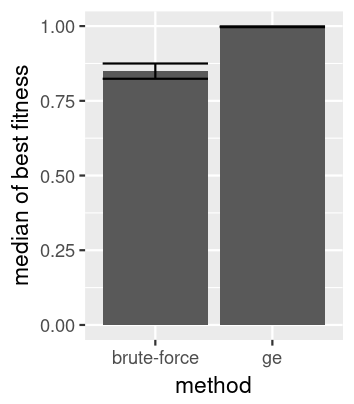
\includegraphics[width=\textwidth]{figures/ge-random}
        \caption{Mean of best fitness}
        \label{fig:ge-random}
    \end{subfigure}
    ~
    \begin{subfigure}{0.4\textwidth}
        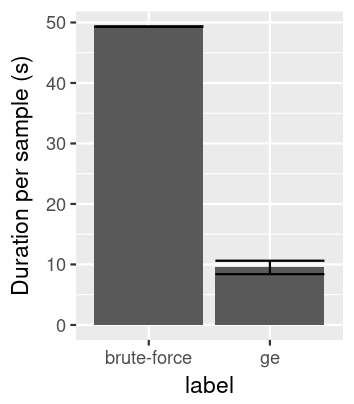
\includegraphics[width=\textwidth]{figures/ge-random-duration}
        \caption{Mean duration}
        \label{fig:ge-random-duration}
    \end{subfigure}
    \caption{GE and random performance compared}
\end{figure}

\section{Evaluation of Evaluation Module}
\subsection{Method}
\subsection{Implementation}
\subsection{Results}
